\chapter{Sequence Digrams}
This section of the thesis contains all sequence diagrams that were created during the design phase during iterative development. Note that schema does not show communication between objects, as usually a sequence diagram does, but it shows communication between the content script, the background script, the native application and the GnuPG application.

There were created three diagrams. The first diagram shows communication between the content scripts of the \textit{OpenPGP.js} prototype (Section \ref{prototype:OpenPGPjs}) and \textit{OpenPGPjs} library (Section \ref{text:openpgpjs}). The second diagram shows a simplified schema of communication between the components of the web browser extension in the implemented \textit{GnuPG\_Decryptor prototype} and can be seen on the figure \ref{img:gnupg_decryptor-sequence}. Next diagram shows an example of decrypting too large content. This feature was implemented in the \textit{Large content prototype} (Section \ref{sec:largeContent}) and can be seen on the figure \ref{img:largeContent}. The last diagram (Figure \ref{img:messageExample}) is an example of the communication between the components of the web browser extension after updating the messaging system in the last iteration of developement process (Section \ref{prototype:finalProduct}).

\begin{figure}[H]
    \begin{center}
        \label{img:openpgp-sequence}
        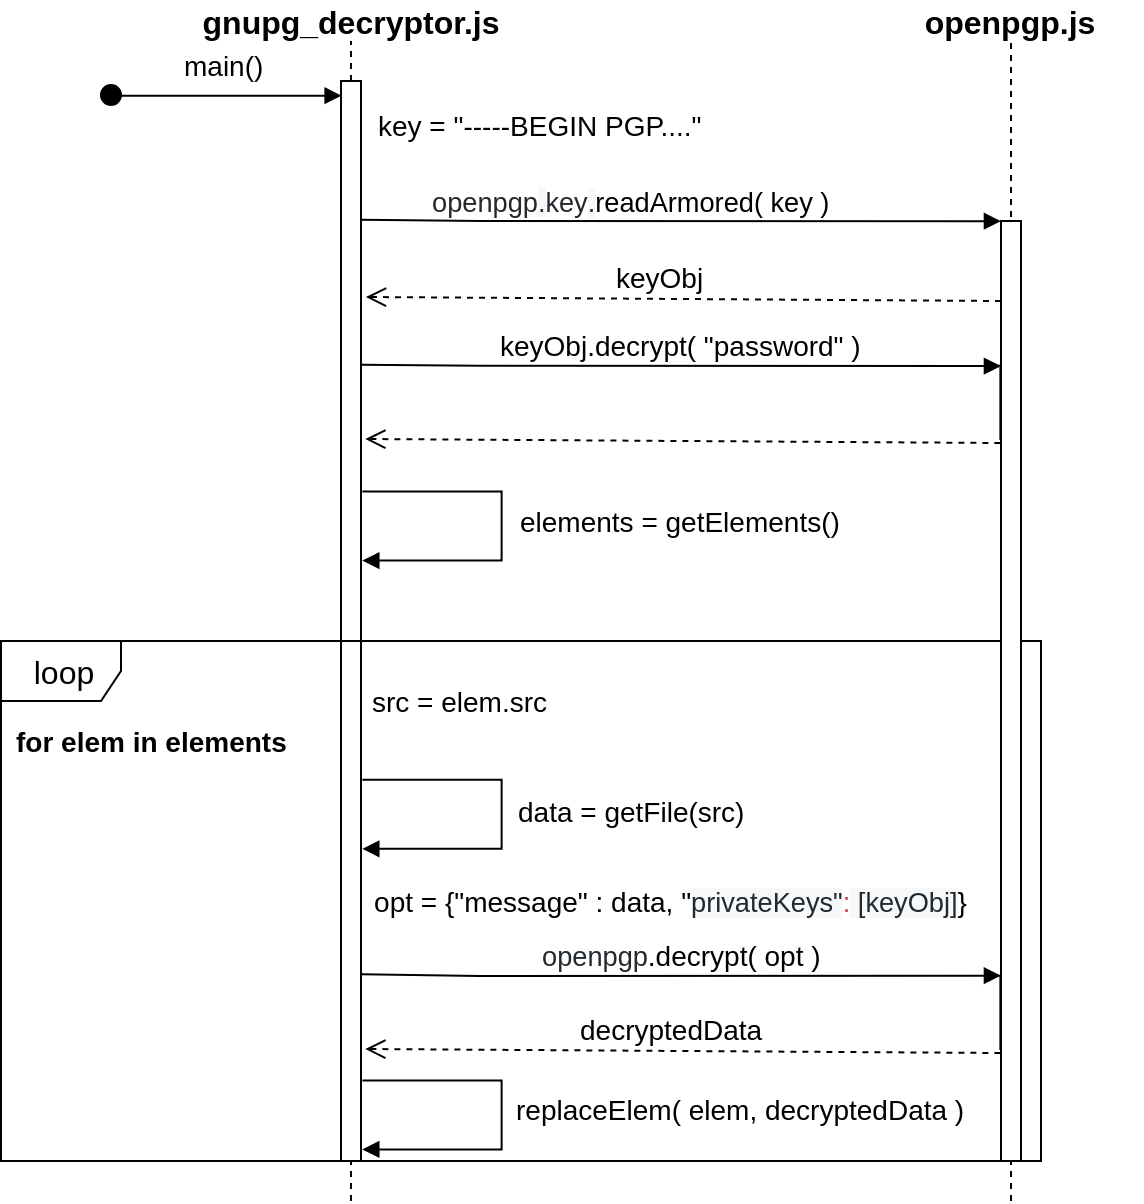
\includegraphics[width=1.3\textwidth,angle=90]{obrazky-figures/openpgp-sequence.png}
        \caption{Communication between the content scripts of \textit{OpenPGP.js} prototype.}
    \end{center}
\end{figure}


\begin{figure}[H]
    \begin{center}
        \label{img:gnupg_decryptor-sequence}
        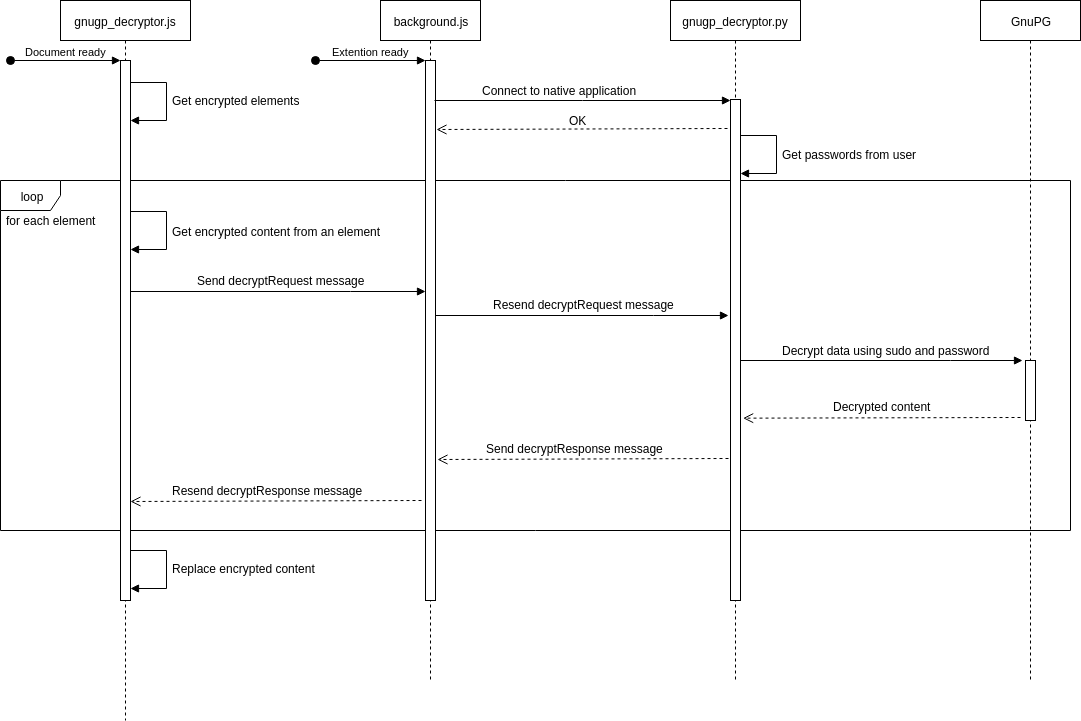
\includegraphics[width=1.3\textwidth,angle=90]{obrazky-figures/sequence-gnupg_decryptor.png}
        \caption{Communication between the web extension, the native application, and the GnuPG application.}
    \end{center}
\end{figure}

\begin{figure}[H]
    \begin{center}
        \label{img:largeContent}
        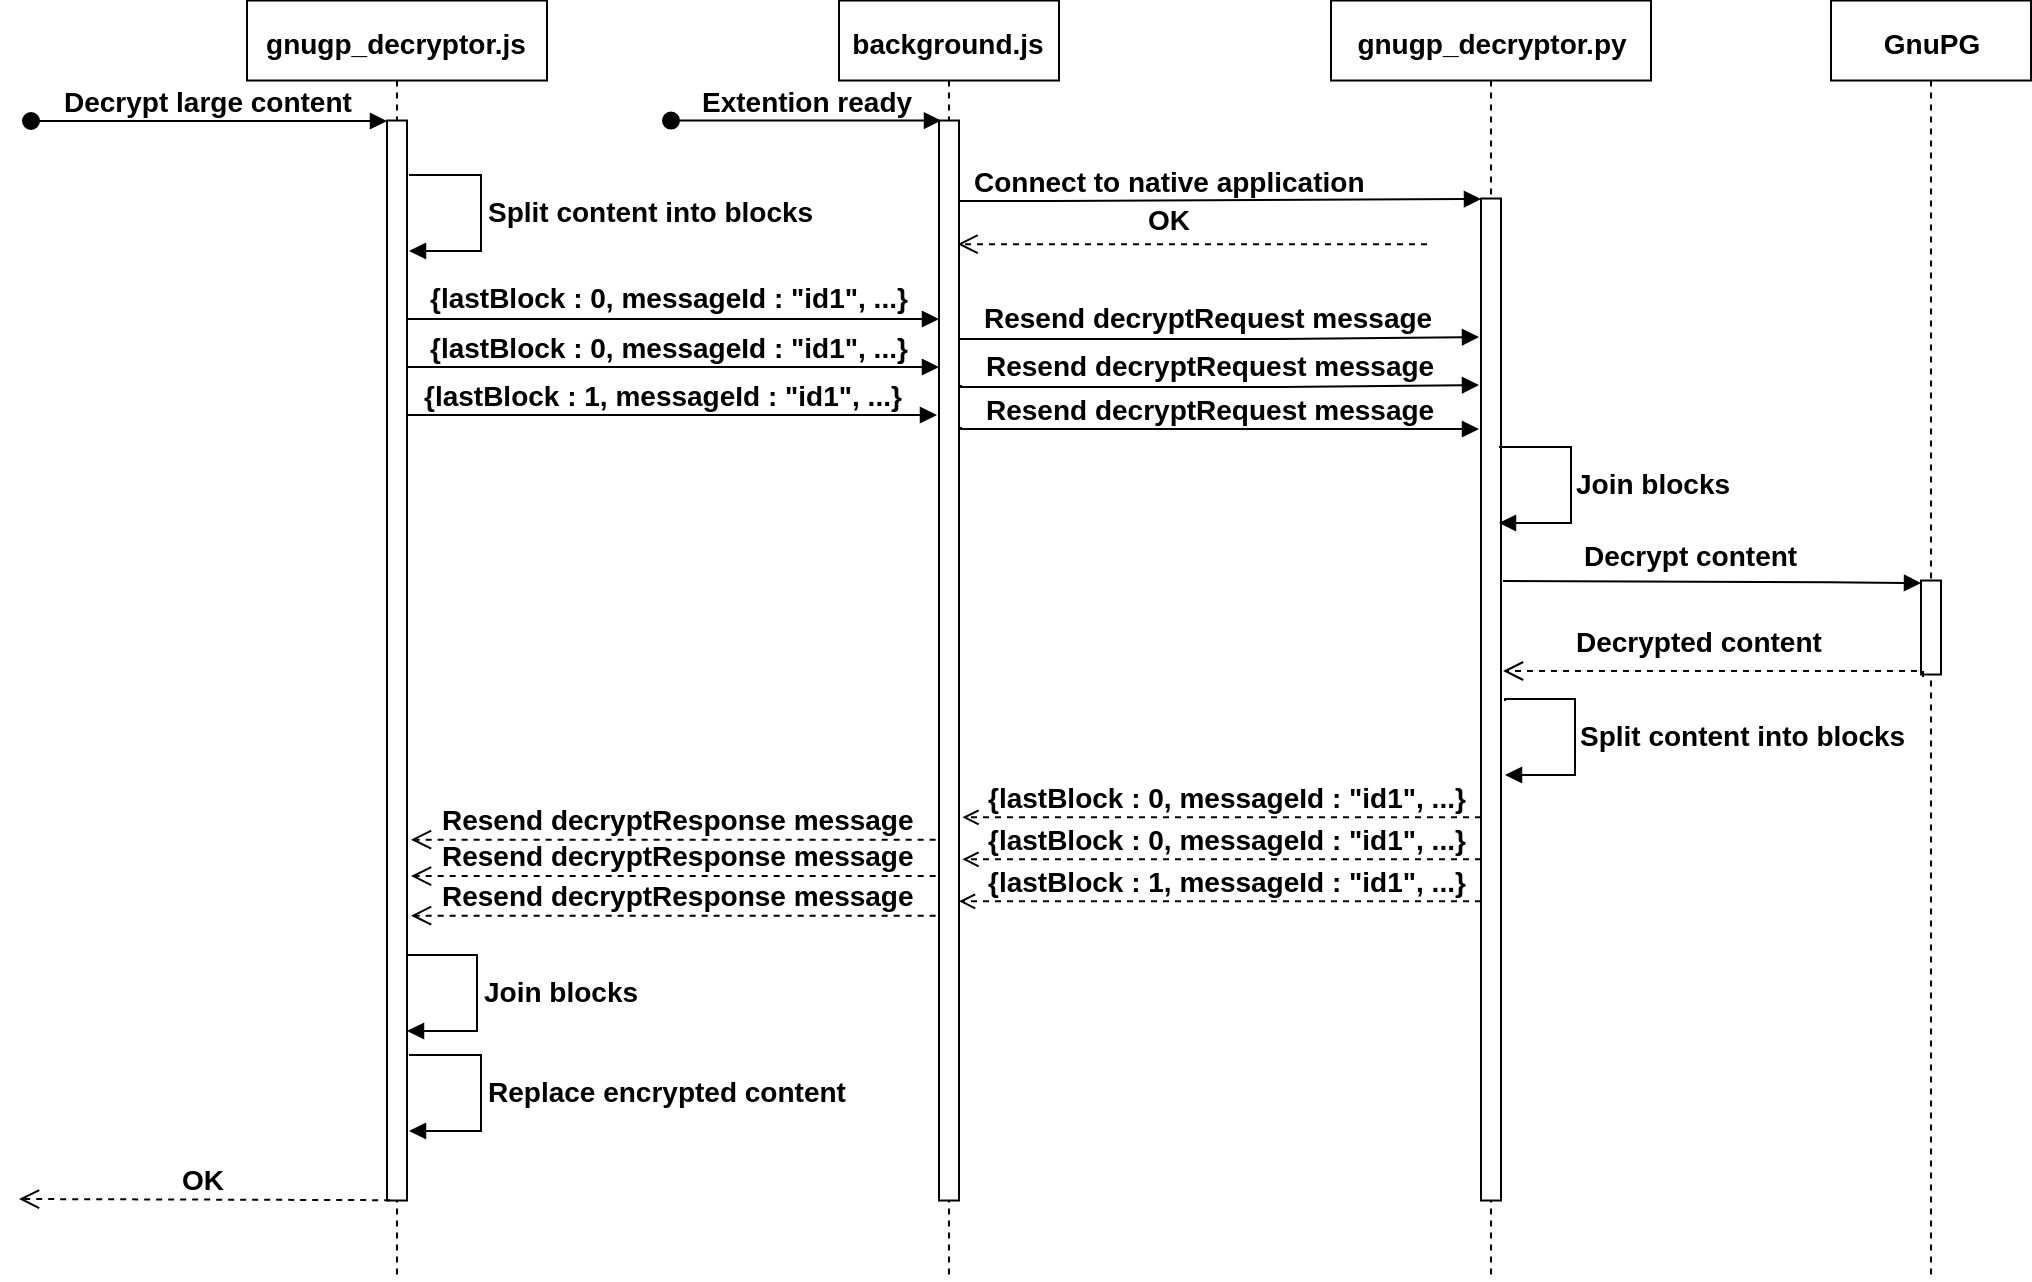
\includegraphics[width=1.3\textwidth,angle=90]{obrazky-figures/sequence-messageDesign.png}
        \caption{An example of decrypting too large content to be sent in a single message.}
    \end{center}
\end{figure}

\begin{figure}[H]
    \begin{center}
        \label{img:messageExample}
        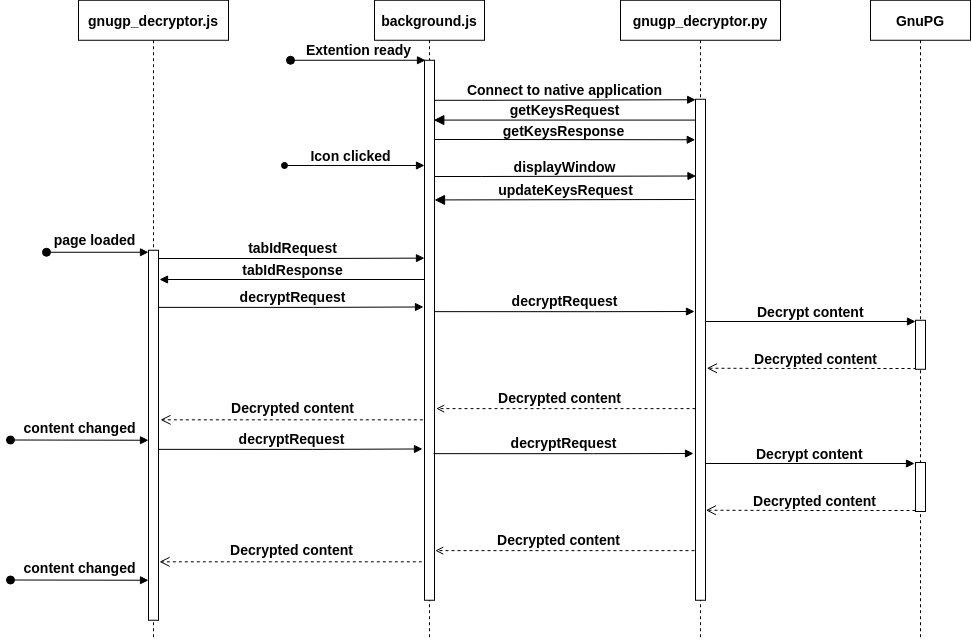
\includegraphics[width=1.3\textwidth,angle=90]{obrazky-figures/sequence-messageExample.png}
        \caption{An example of communication between the components of the web browser extension.}
    \end{center}
\end{figure}

\chapter{Contents of the Attached StorageMedia}
On the attached storage media, the following files can be found:

\begin{itemize}
    \item The digital form of the thesis,
    \item \LaTeX source codes of the thesis,
    \item the GnuPG Decryptor extension,
    \item the native application for the GnuPG Decryptor extension,
    \item implemented prototypes,
    \item mplemented test pages (without encrypted audio and video files),
    \item GPG public and private keys,
	\item README file with password for keys and the description of the content.
\end{itemize}

